\section{Analysis}
\label{sec: analysis}

\subsection{Feature Analysis}

The first thing we want to answer in this paper is about browser features, feature trends, and feature lifespan. We extracted number of features in each browser version from our dataset. Then by comparing the feature set between different versions we find out how many features are added and removed from each version. We see that Chrome is Adding and removing much more features compared to firefox. But firefox removes bigger portion of its features in each version.

\ali{Add data about feature lifespans}

\begin{figure}[ht]
    \centering
    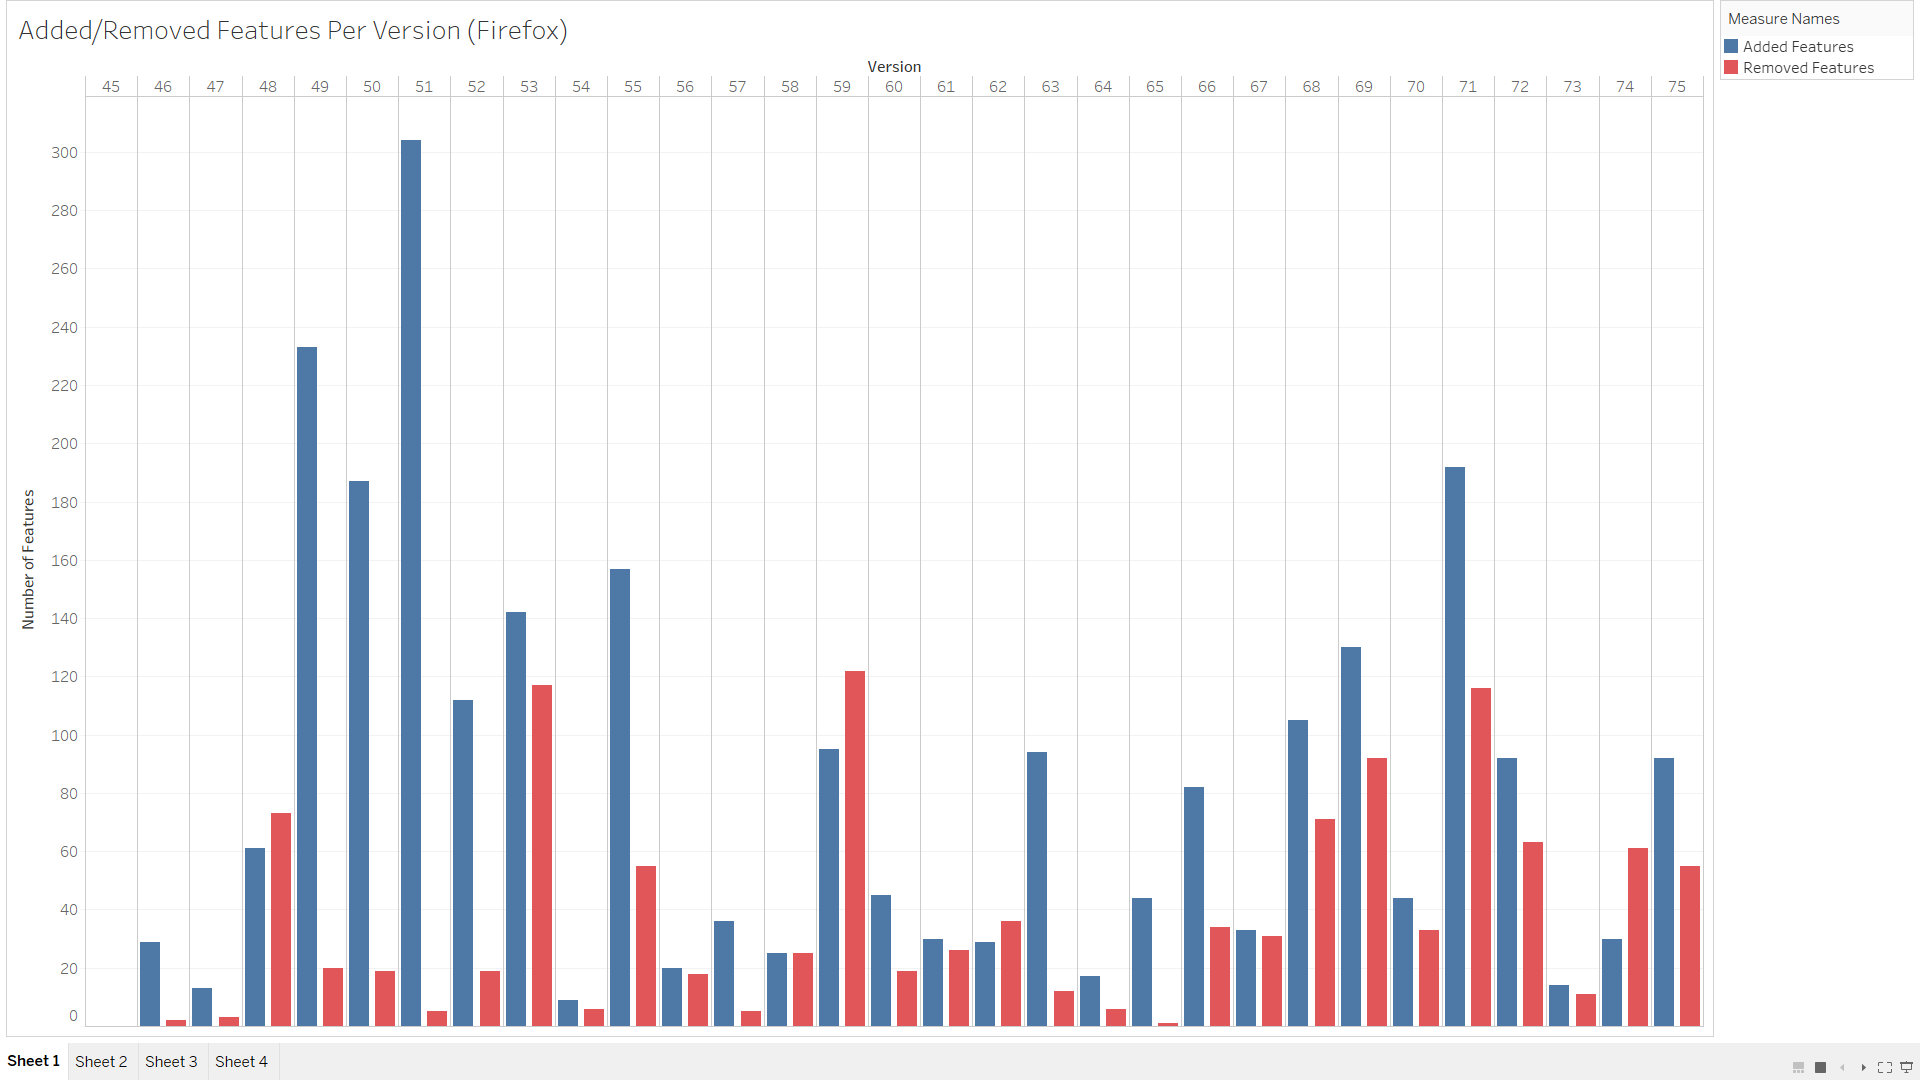
\includegraphics[width=\columnwidth]{figures/Firefox-add-remove.png}
    \caption{Feature Introduction and removal in Firefox. Red bars represent the removed features and the blue bars represent added features.}
    \label{fig:times_bar}
\end{figure}


\begin{figure}[ht]
    \centering
    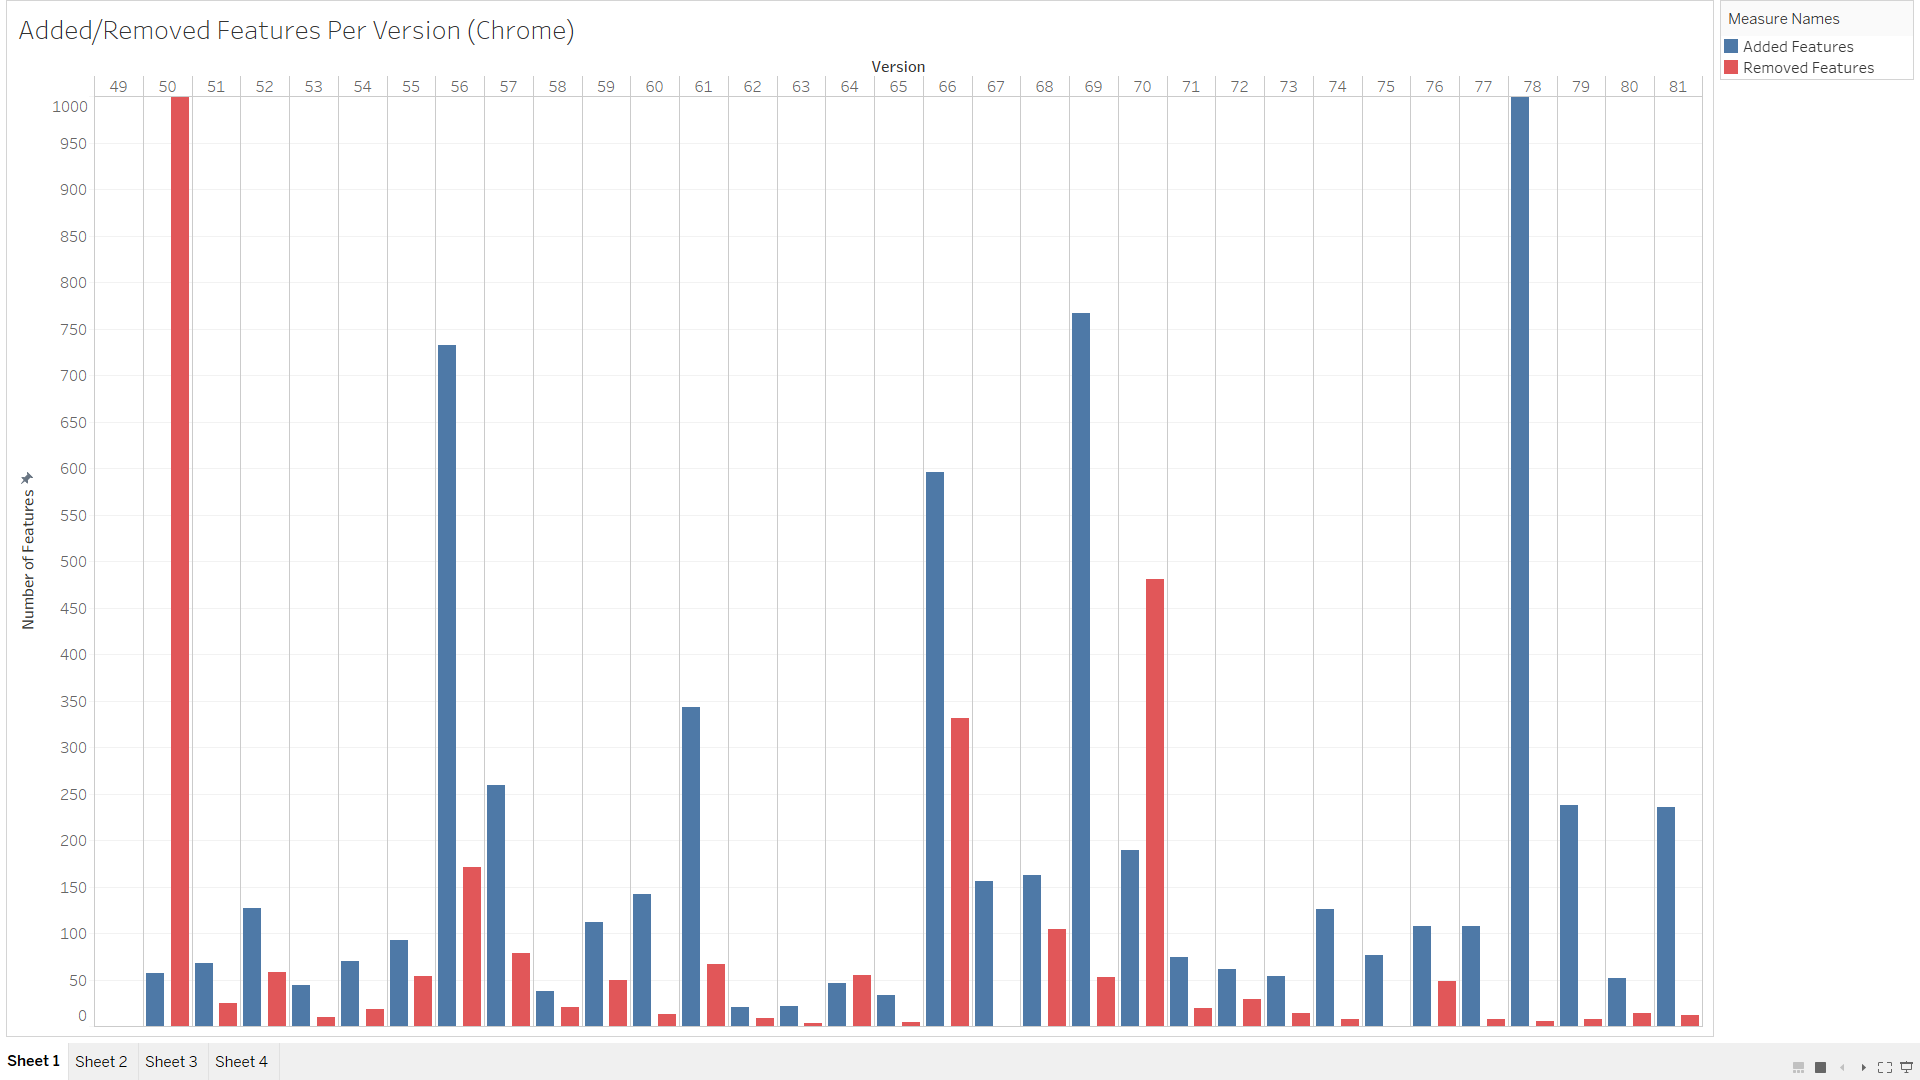
\includegraphics[width=\columnwidth]{figures/Chrome-add-remove.png}
    \caption{Feature Introduction and removal in Chrome. Red bars represent the removed features and the blue bars represent added features.}
    \label{fig:times_bar}
\end{figure}

By using the extracted data for the previous part, we tried to compare feature trends in Chrome and Firefox. We see that Chrome is adding much more features to its browsers comparing to Firefox. Firefox tries to keep its features number more steady. They try to remove bigger portion of their feature set in each version. We cannot say one of them is following the other one in terms of feature introduction and removal.

\begin{figure}[ht]
    \centering
    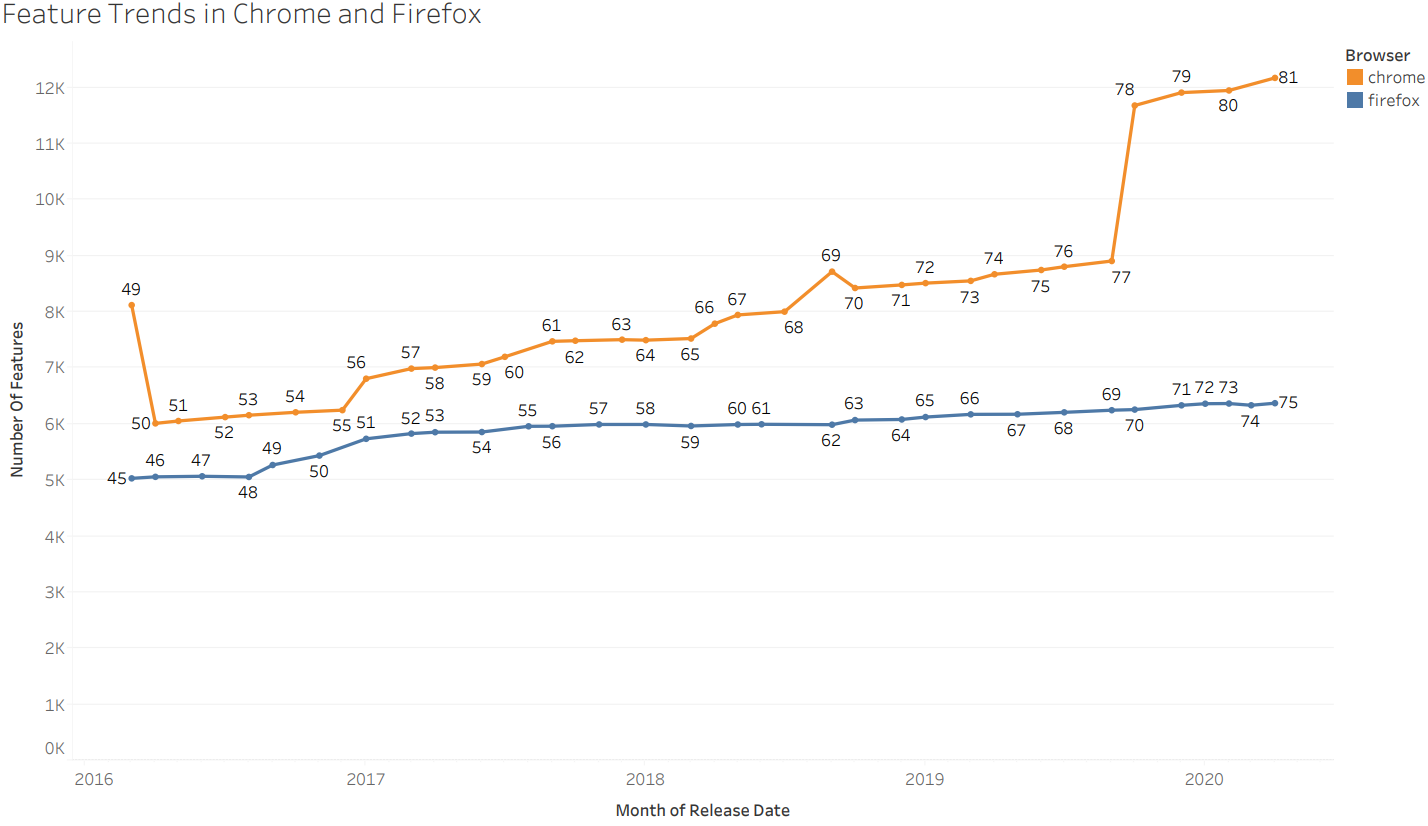
\includegraphics[width=\columnwidth]{figures/Feature-Trends.PNG}
    \caption{Feature trends in firefox and chrome. Blue line represents number of features in chrome. Yellow line represents firefox.\ali{Need to rescale the chart so the text could be visible}}
    \label{fig:times_bar}
\end{figure}



\subsection{Browser Fingerprintability}
We wanted to answer two different things about browser fingerprinting in our paper. The questions are as follows. Can we say that all browsers are fingerprintable? Are browsers becoming more fingerprintable?

To answer the first question, we created a feature set for each browser version that we had. A feature set is a set of browser features that exist in a specific browser version. After creating the feature set for each browser version in our study, we compared these sets to each other and realized that all of these sets are unique. This means that there are no two browsers that have the same feature set. This means that all of these browsers are fingerprintable. The reason for this finding is that browser vendors keep removing and adding features to their newer versions so that the feature set for each version becomes different than the others. So the answer to our question is yes. All of the browser versions in our study were fingerprintable.


In order to answer the second question, we tried to compare the feature sets to each other. We see that vendors specially Google Chrome are adding lots of features to their newer versions but they do not remove features as much as they add. We see that the feature set for each browser is converging and we are tending to homogeneity of browser features. The unique feature set is getting smaller in almost every new browser version. The unique feature set is the set of features which make a specific browser version unique; either by being in the feature set or by not being in the feature set. \ali{maybe explain this more}
So based on our findings, we cannot say that browsers are becoming more fingerprintable. Actually, they are becoming less fingerprintable.

\ali{Mention the size of the smallest and biggest feature set}

\ali{Generate a chart to show this finding}


\subsection{Vulnerability Analysis}
We have not been able to find a relation between number of vulnerabilities in a browser and number of features inside it. As we saw earlier, the number of features is increasing in newer browser version. But we saw that number of vulnerabilities is decreasing because newer browsers are becoming more secure by fixing security issues that existed in older browser version. Also, there may be undetected vulnerabilities in newer browsers which makes the vulnerability set smaller. So we cannot confidently say that there is a relation between number of features and number of vulnerabilities in browsers.

\ali{Still need to generate results and reports for this section.}